\documentclass[letter,10pt]{article}
\usepackage[utf8]{inputenc}
\usepackage[spanish, activeacute]{babel}
\usepackage{float}
\usepackage{geometry}
\geometry{verbose,tmargin=0cm,bmargin=2cm,lmargin=2cm,rmargin=2cm,headheight=0cm,headsep=1cm,footskip=1cm}
\usepackage{graphicx}


%%%%%%%%%%%%%%%%%%%%%%%%%%%%%% Textclass specific LaTeX commands.
\newcommand{\lyxaddress}[1]{
\par {\raggedright #1
\vspace{1.4em}
\noindent\par}
}

%%%%%%%%%%%%%%%%%%%%%%%%%%%%%% User specified LaTeX commands.
\date{}

\begin{document}

\title{Problema A - Annie la Hija de la Obscuridad}


\includegraphics[scale=0.6]{logo} \hspace*{9.00cm}

\includegraphics[scale=0.5]{dsc} 
\bigskip
\begin{center}
	\Large Problema A - Annie la Hija de la Obscuridad
\end{center}

\begin{flushright}
Límite de tiempo: 3 segundos
\par\end{flushright}
\bigskip

\section*{Problema}

League of Legends es un videojuego de género MOBA, desarrollado por Riot Games para Microsoft Windows y OS X.

Los jugadores (invocadores), se agrupan en 2 equipos de campeones (champions, o bien champs), 3 vs 3 o 5 vs 5. A partir de diciembre del 2013 hay 118 campeones disponibles en los servidores normales, pero este número aumenta periódicamente. Cada equipo comienza en lados opuestos de un mapa en un área llamada Base, cerca de lo que se llama Nexo (o Nexus). El objetivo del juego es destruir el Nexo del equipo rival. Para destruir un nexo, cada equipo debe llegar a la base enemiga eliminando unas torretas que la protegen.

Cada jugador gana niveles al matar súbditos (NPCs que aparecen constantemente y atacan al otro equipo) del equipo contrario y derrotar a monstruos neutrales. Matar monstruos, campeones enemigos y destruir torretas proporciona oro necesario para mejorar al Campeón y facilitar así las batallas.

\begin{figure}[H]
\centering
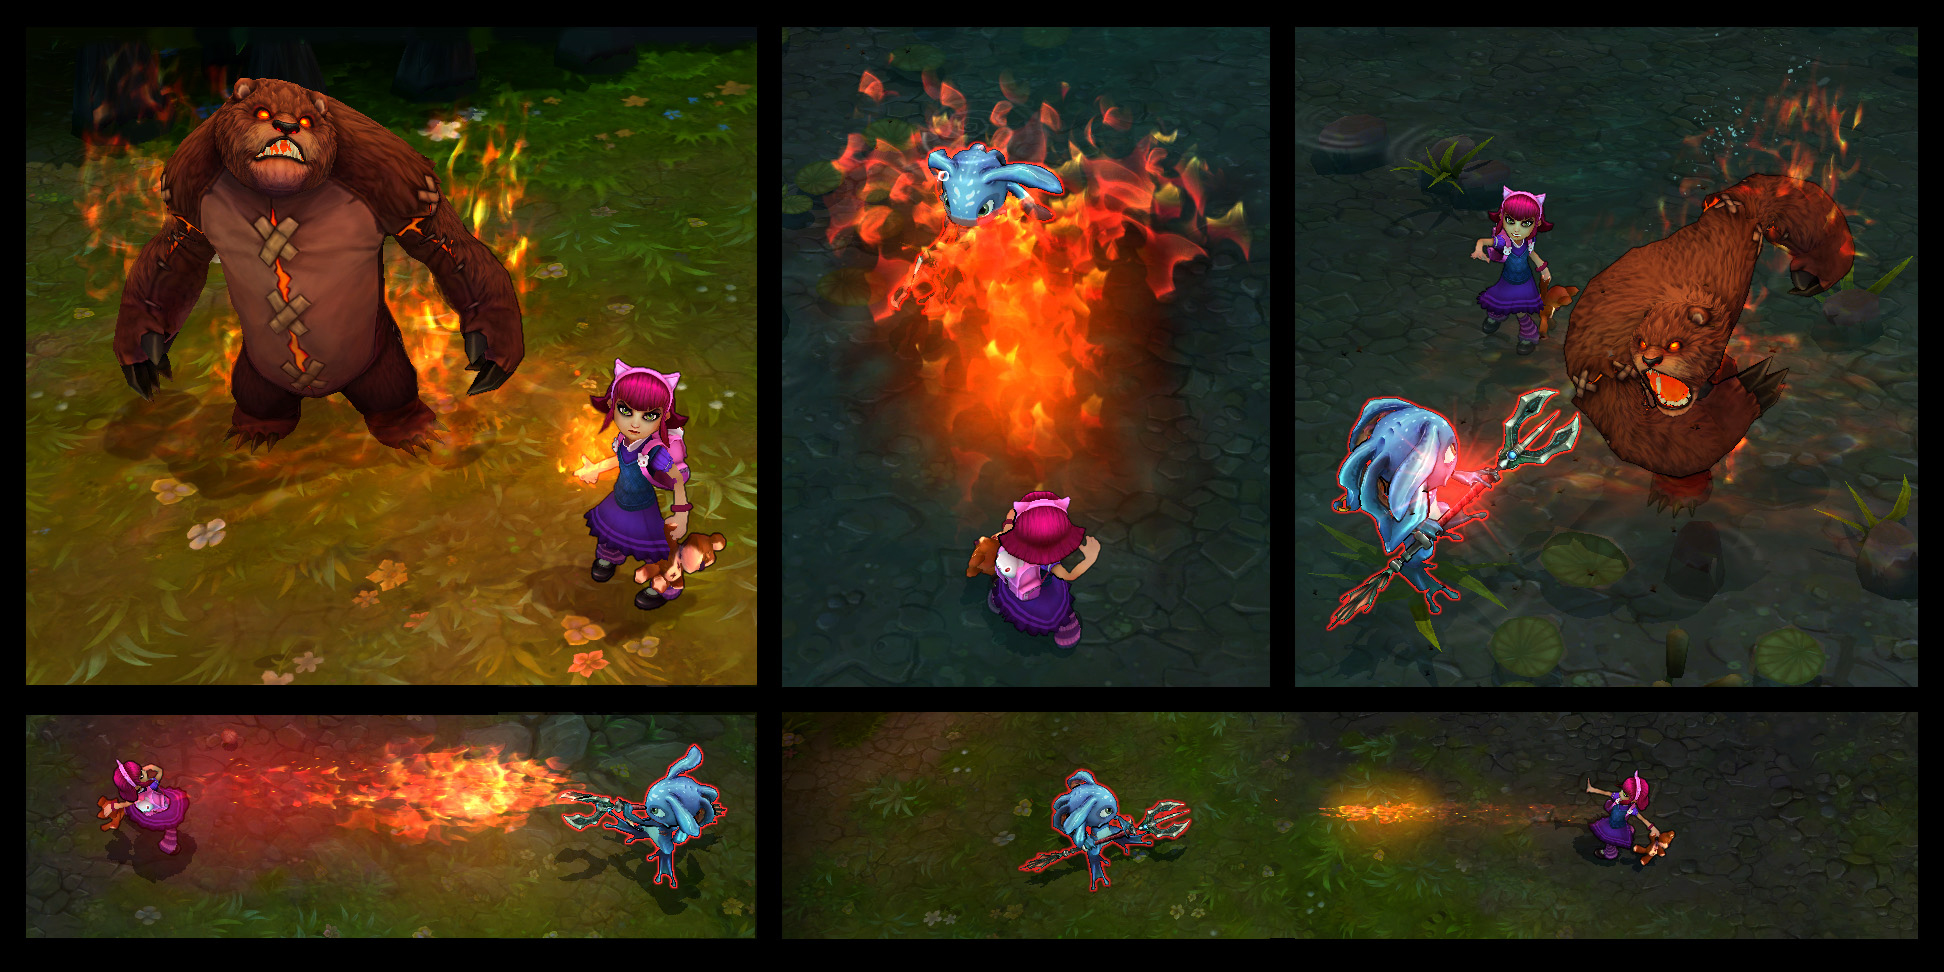
\includegraphics[keepaspectratio=true,scale=0.2]{Annie_comic.jpg}
\caption{Arriba a la izquierda ``Tibbers'', arriba al centro ``Incinerar'', Abajo a la 
izquierda ``Desintegrar''}
\label{fig:my_label}
\end{figure}

Uno de estos champs es Annie, tu objetivo es ayudarla a determinar cuando podrá 
encadenar sus tres hechizos ofensivos a un campeón enemigo. Los hechizos que conoce Annie son los siguientes:
\begin{itemize}
\item ``Desintegrar'' Annie lanza una bola de fuego imbuida de Maná a cualquier campeón en un area de $600 u$ \footnote{$u$ son unidades de longitud en los campos de la justicia} a su alrededor.$$$$$$$$
$$$$$$$$$$$$$$$$
$$$$$$$$

\item ``Incinerar'' Annie lanza un abrasador cono de fuego, dañando a todos los enemigos de la zona. Este cono tiene una apertura de $35^o$  y además tiene un 
alcance de $500u$ (imagine una rebanada de pizza circular, con centro en Annie).

\item ``Invocar: Tibbers'' Tibbers aparece en un estallido de llamas e inflige 
daño mágico a los enemigos en la zona objetivo. Annie puede invocar Tibbers en 
cualquier lugar a no más de $700u$, Tibbers inflinge daño de area donde aparece en
un círculo de radio $75u$.
\end{itemize}

Puedes asumir de manera segura que no hay obstáculos entre Annie y su objetivo; además
puedes despreciar el tiempo entre el lanzamiento de cada hechizo.

\subsection*{Entrada}

La primer línea de la entrada será un número $2 \leq T \leq 20$ que será el número de casos.
Cada caso comenzará con tres números $ 0 \leq A_x , A_y \leq 10000$ y $1 \leq Q \leq 50$ donde los primeros dos son 
las coordenadas de Annie y el tercero el número de consultas para ese caso.
Las siguientes $Q$ líneas tendrán dos números $ 0 \leq E_x,  E_y  \leq 10000$ que es la posición de el 
campeón objetivo.
Se  asegura que todos los números en la entrada son enteros.

\subsection*{Salida}

Para cada consulta deberas imprimir una línea que dirá ``FULL COMBO'' si puedes 
encadenar los 3 hechizos contra el campeón objetivo al mismo tiempo, si no puede, imprime 
``OUTPLAYED''.

\subsection*{Entrada Ejemplo}

\begin{verbatim}
2
0 1 1
490 2
23 4 1
700 900 
\end{verbatim}

\subsection*{Salida Ejemplo}

\begin{verbatim}
FULL COMBO
OUTPLAYED
\end{verbatim}

\subsection*{Sugerencias}

$c^2 = a^2 + b^2$

\noindent \rule[0.5ex]{1\columnwidth}{1pt}


\lyxaddress{Edgar García Rodríguez-Grupo de Algoritmia Avanzada y Programación Competitiva}
\end{document}
